\documentclass[11pt,a4paper]{article}

\usepackage[T1]{fontenc}
\usepackage[utf8]{inputenc}
\usepackage[english]{babel}
\usepackage{graphicx}
\usepackage{varioref}
\usepackage{color}
\setlength\parindent{0pt}
\usepackage{amsmath}
\usepackage{geometry}
\usepackage{amssymb}
\geometry{hmargin=3cm}
\usepackage{amsthm}
\usepackage{mathtools}
\usepackage{epstopdf}
\usepackage{subfigure}

\newtheorem{theorem}{Theorem}

\begin{document}

\title{LINMA2111 - CM2 - 2015}
\author{Mathieu Dath \& Damien Scieur}
\date{\today}
\maketitle

In the last course, we have seen the QuickSort algorithm (Hoare, 1962). This algorithm is often used in practice due to the low constant in its complexity. We have also seen that there is some randomness in this algorithm. One may now wonder if there is a deterministic algorithm in $\mathcal{O}(n\log n)$ (worst case complexity) which sorts "in place" (meaning that it uses no extra memory. 
\\ \\
Fortunately for the people who really hate randomness, the answer is yes, but we need to be smart about the way we keep track of the information. In other words, we need a good data structure.

\subsubsection*{Stack v.s. Queue}


Let us make a little digression about two well studied data structures, stacks and queues. Both are ordered lists of entries with the same static structure but different ways to access/modify it. The difference is graphically explained on Figure \ref{stackandqueue}.

\begin{figure}[!h]
	\centering
 	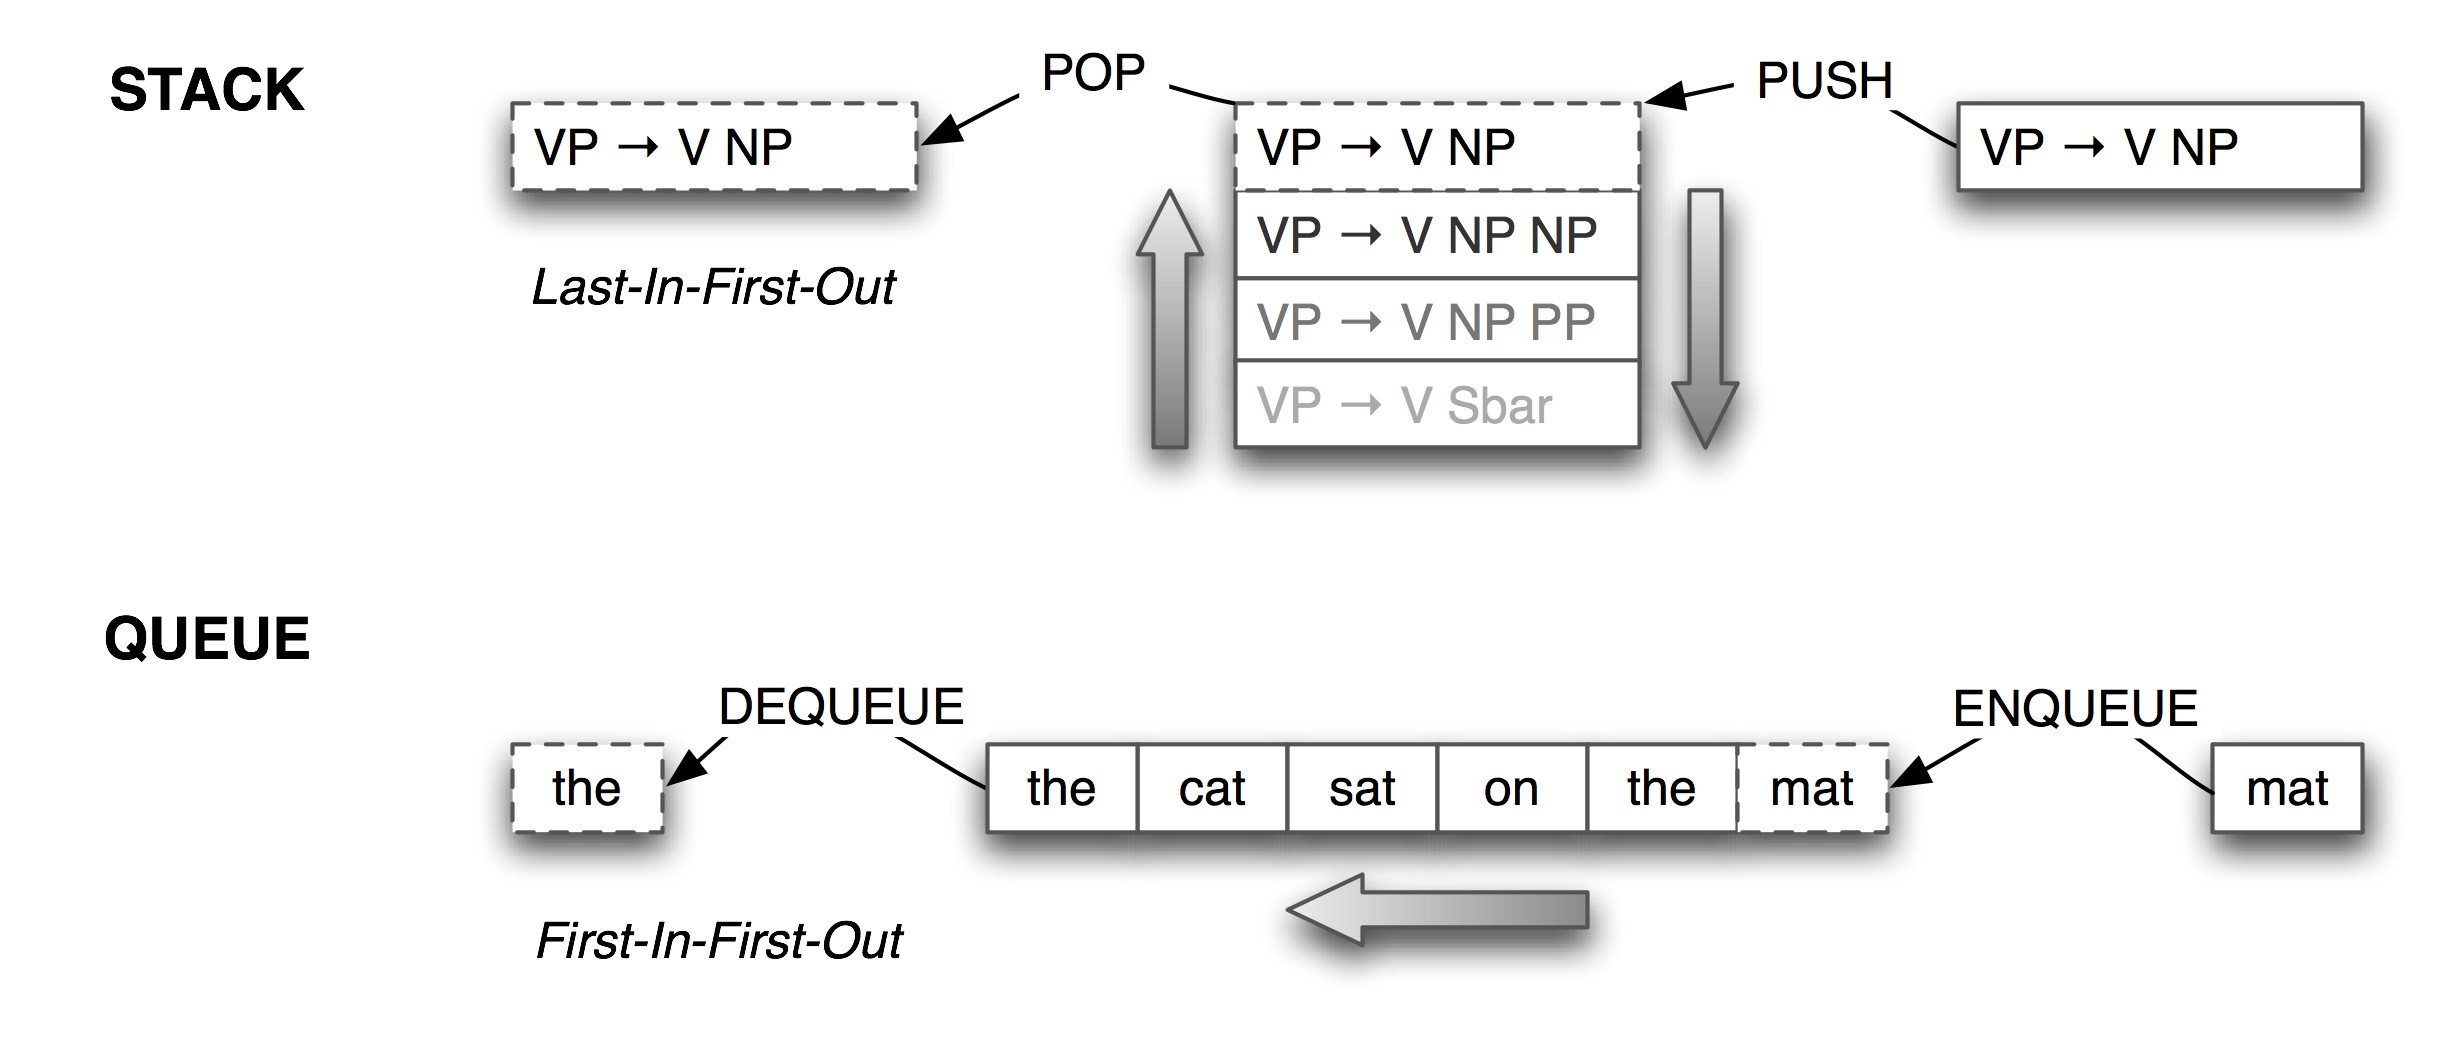
\includegraphics[width=0.9\textwidth]{stack-queue.png}
  	\caption{Graphic representations of the stack and the queue structures. Elements are inserted using the Push/Enqueue action and removed using the Pop/Dequeue action.}
   	\label{stackandqueue}
\end{figure}

We define a data structure as a static structured set (like a list, a tree, etc.) with a list of operations (like read, insert, etc.). It can thus be seen as an abstract mathematical concept. 

\subsection*{A data structure for a deterministic QuickSort}

If we get back to our problem, the structure we need is a priority queue: a set of numbers with the following operations:
\begin{itemize}
\item Insert
\item Extract Max
\end{itemize}

An example of the use of such a structure is a todo list where the elements are tasks and where each task is assigned a priority (which can be interpreted as a number). 
\\ \\
If we have an implementation for a priority queue, then we have a sorting algorithm for $\left[ \text{T(1)} \; \text{T(2)} \; \cdots \; \text{T(}n\text{)} \right]$, we just need to:
\begin{enumerate} 
\item Insert T(1), T(2), ..., T($n$) to an empty priority queue.
\item Extract Max $n$ times
\end{enumerate}
The complexity of such an algorithm is $n \left( \text{cost(Insert)} + \text{cost(Extract Max)} \right)$.

\subsubsection*{Potential structures for this sorting algorithm}

We need a data structure to implement the sorting algorithm algorithm we just described. 

\paragraph*{Unordered table} Using an unordered table, the operations complexity are \begin{itemize}
\item Insert: $\mathcal{O}(1)$
\item Extract Max: $\Theta (n)$
\end{itemize}
The sorting algorithm associated to this implementation has thus the complexity $\Theta (n^2)$. \newline
$\Rightarrow$ This is SelectionSort.

\paragraph*{Ordered table} Using an ordered table, the operations complexity are \begin{itemize}
\item Insert: $\mathcal{O}(n)$ \textit{$[$cost of shifting the entries$]$}
\item Extract Max: $\mathcal{O}(1)$
\end{itemize}
The sorting algorithm associated to this implementation has thus the complexity $\mathcal{O} (n^2)$. \newline
$\Rightarrow$ This is InsertionSort.

\paragraph*{"Heap"} Using a heap, the operations complexity are \begin{itemize}
\item Insert: $\mathcal{O}(\log n)$
\item Extract Max: $\mathcal{O}(\log n)$
\end{itemize}
The sorting algorithm associated to this implementation has thus the complexity $\mathcal{O} (n \log n)$.

\subsubsection*{Heap structure}

A heap is a tree with the following properties:
\begin{itemize}
\item essentially binary complete (only the last level may be incomplete (as it is filled from left to right))
\item $\text{entry}(x) \leq \text{entry}(\text{father}(x)) \; \forall \; \text{node} \; x \neq \text{root}$
\end{itemize}
An example of a heap is shown in Figure \ref{tree1}.

\begin{figure}[h!]
\centering
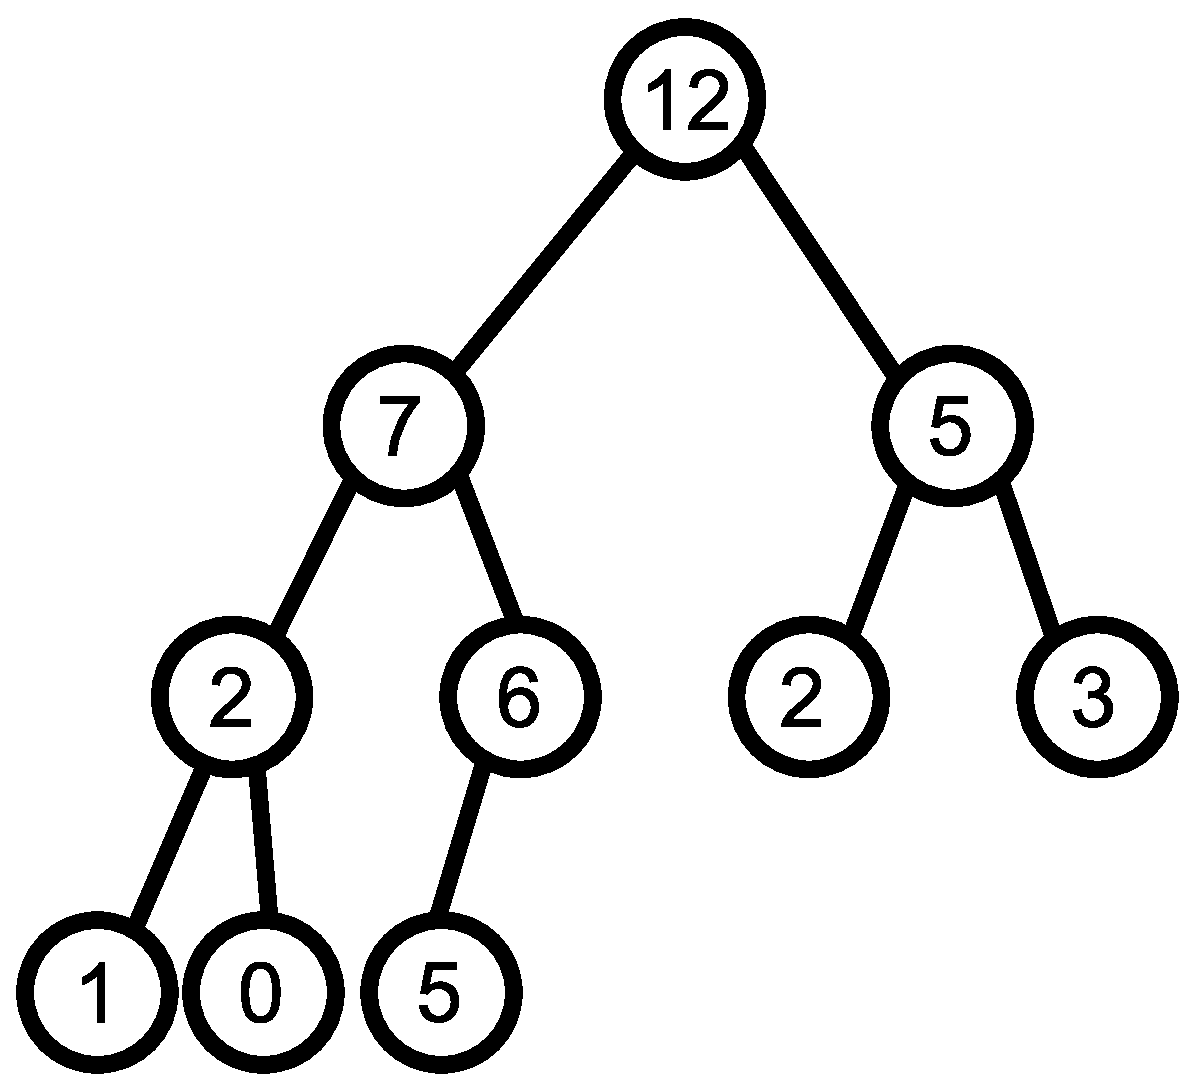
\includegraphics[scale=0.5]{inkscape/tree1.eps}
\caption{Example of a heap}
\label{tree1}
\end{figure}

\paragraph*{Insert} To insert a new node into the heap, add it to the last level in the first free position and swap it with its father until the heap is properly re-established. \newline
$\Rightarrow \mathcal{O}(\log n)$
\\ \\
\begin{figure}[htbp]
\centering
\begin{subfigure}
\centering
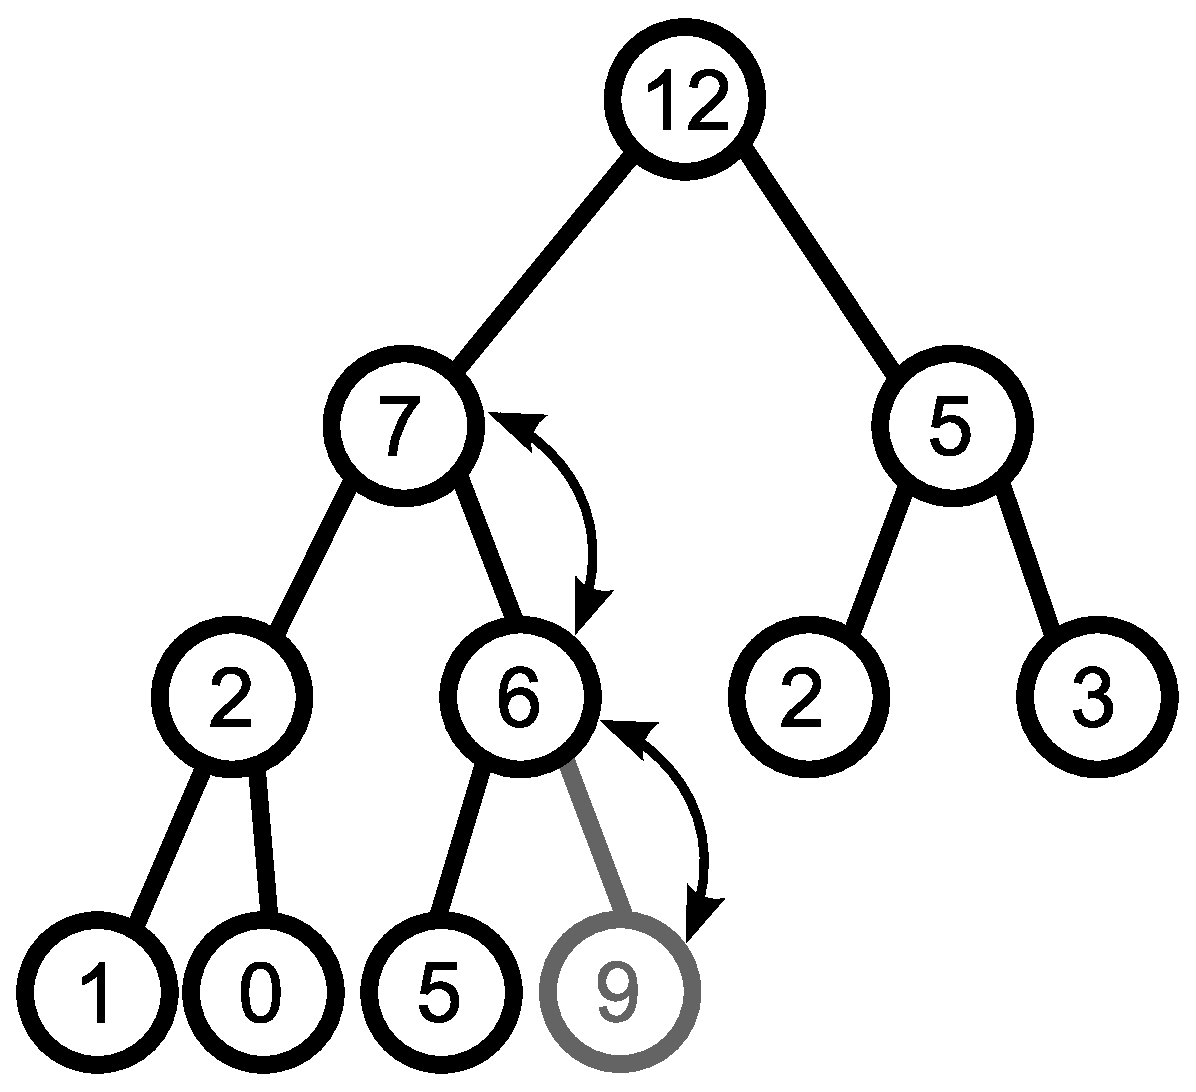
\includegraphics[width=0.45\textwidth]{inkscape/tree2.eps}
\end{subfigure}%
\begin{subfigure}
\centering
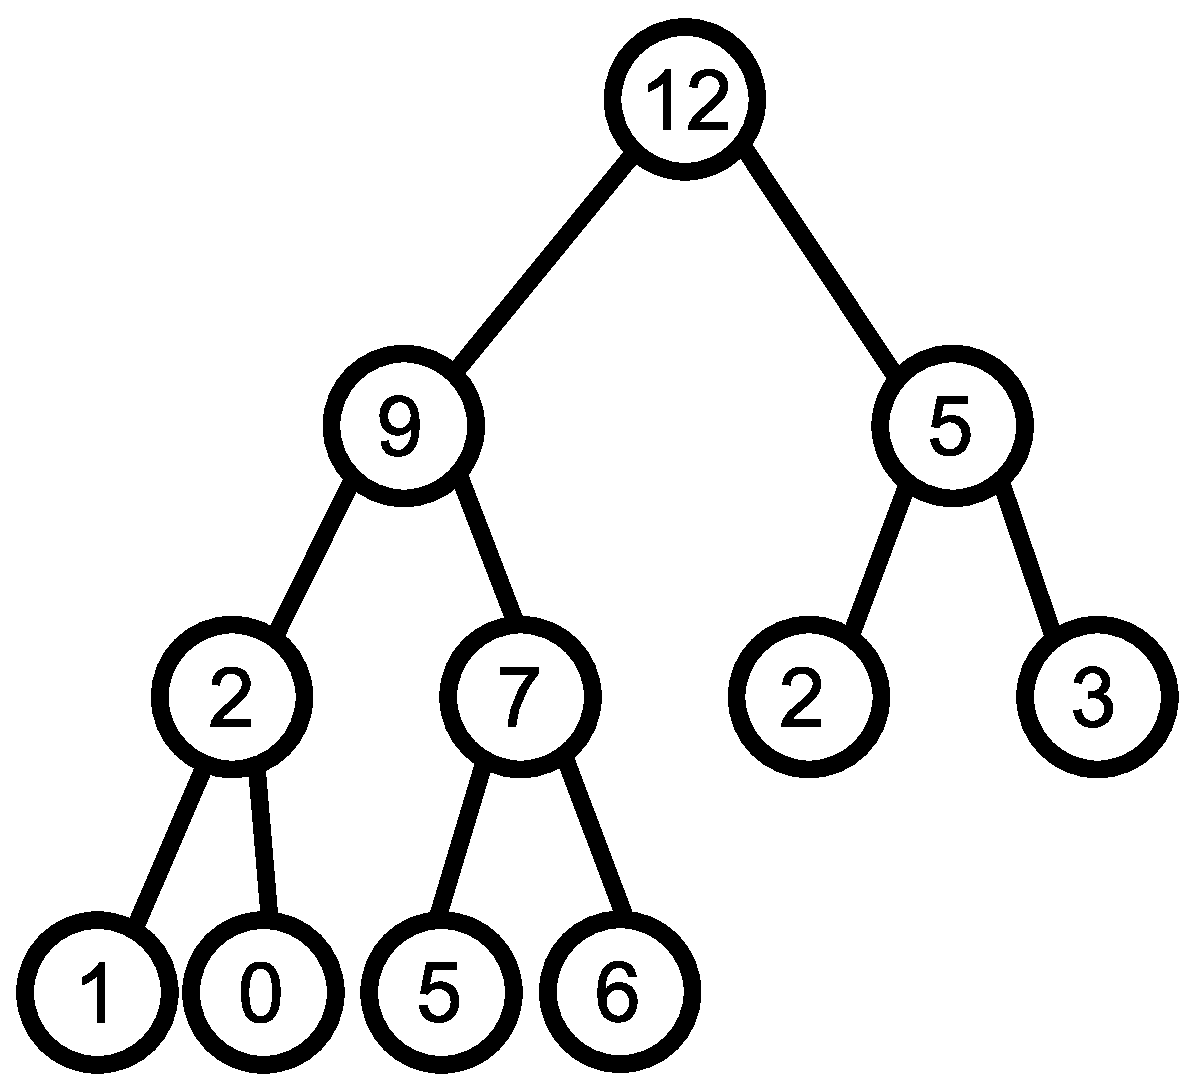
\includegraphics[width=0.45\textwidth]{inkscape/tree3.eps}
\end{subfigure}%
\caption{A heap before/after adding one element}
\label{tree2_3}
\end{figure}

\paragraph*{Extract Max} To extract the maximal node from the heap, one needs to:
\begin{enumerate}
\item Swap root (the max entry) with last entry
\item Remove the max entry
\item Swap new root with its \emph{largest} child until the heap properly is restored.
\end{enumerate}
$\Rightarrow \mathcal{O}(\log n)$
\\ \\

\begin{figure}[htbp]
\centering
\begin{subfigure}
\centering
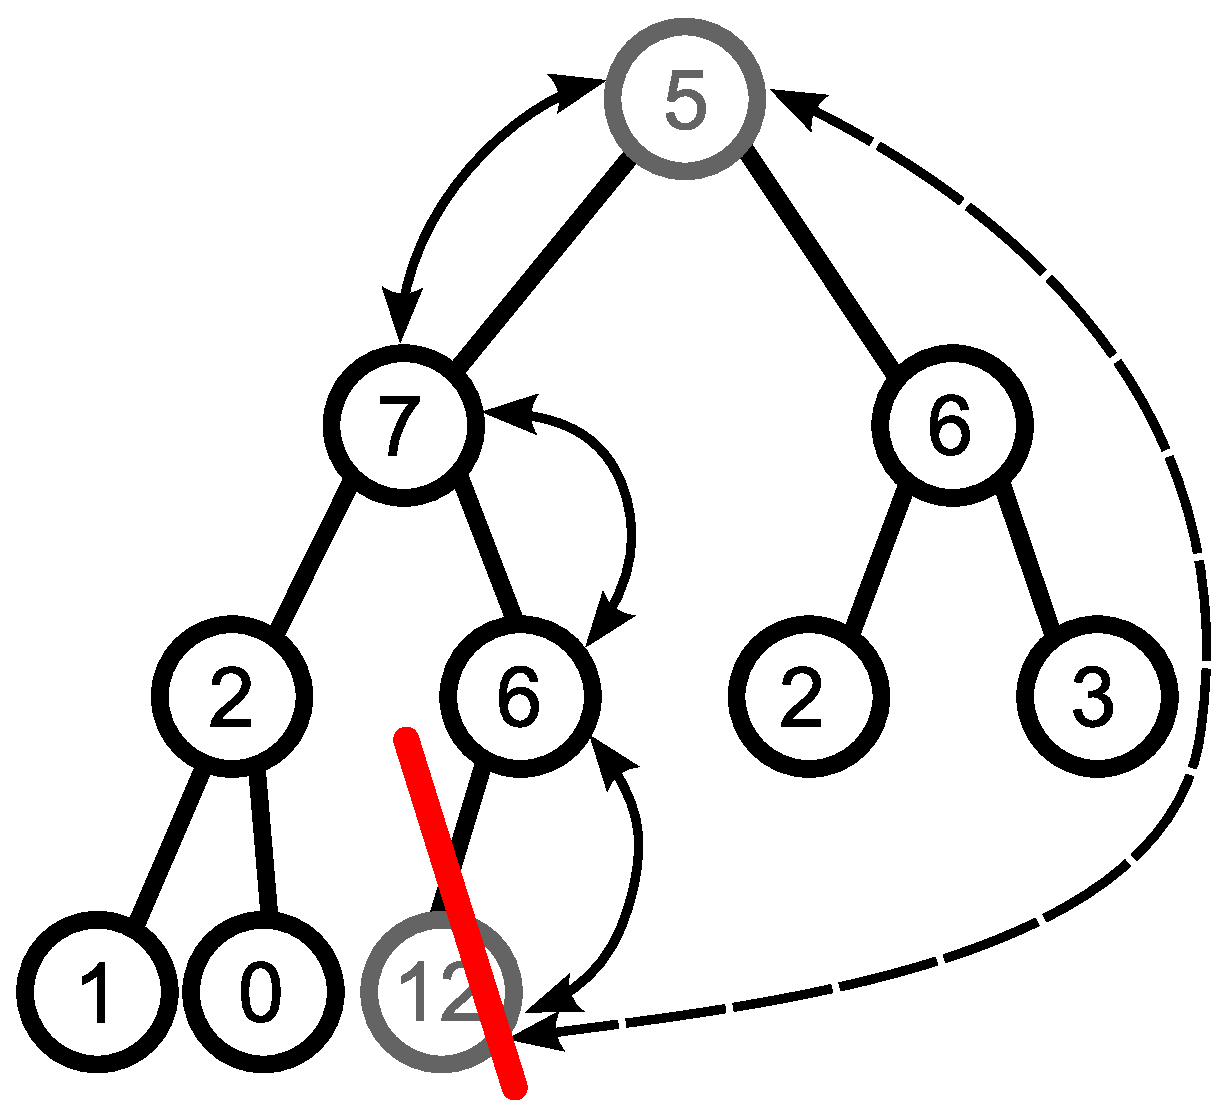
\includegraphics[width=0.45\textwidth]{inkscape/tree4.eps}
\end{subfigure}%
\begin{subfigure}
\centering
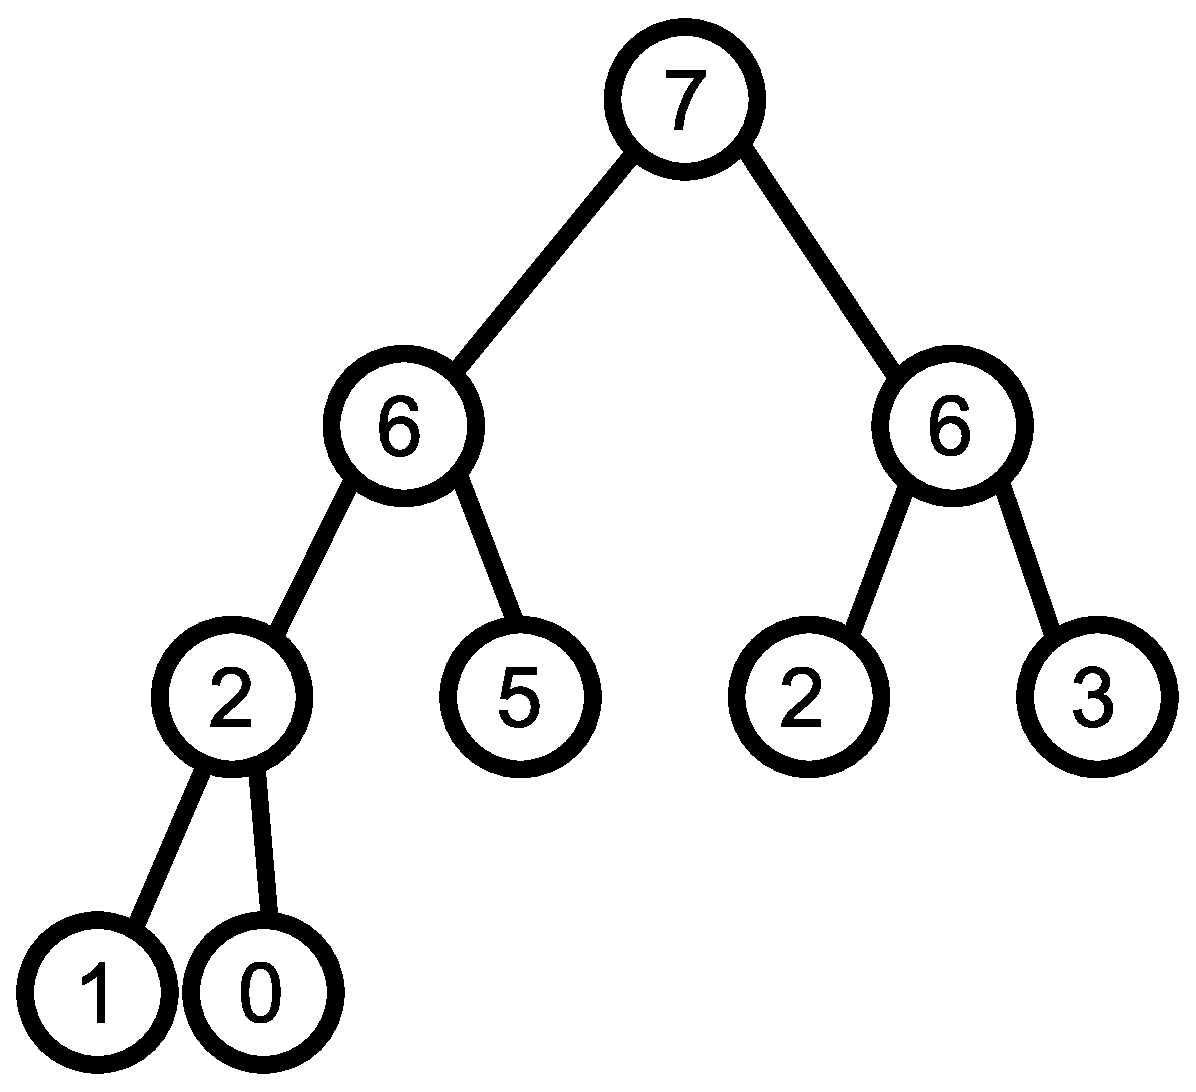
\includegraphics[width=0.45\textwidth]{inkscape/tree5.eps}
\end{subfigure}%
\caption{A heap before/after removing the largest entry}
\label{tree4-5}
\end{figure}
The resulting sorting algorithm is called the HeapSort (Williams, 1964) and has a complexity of $\mathcal{O}(n\log n)$.

\subsubsection*{Remarks}

\begin{itemize}
\item The heap may be stored as an array: \\
\begin{center}
\begin{tabular}{|c|c|c|c|c|c|c|c|c|c|c|}
   \hline
   \textbf{Heap (T)} & 12 & 7 & 6 & 2 & 6 & 2 & 3 & 1 & 0 & 5 \\
   \hline 
   \textbf{Index} & 1 & 2 & 3 & 4 & 5 & 6 & 7 & 8 & 9 & 10 \\
   \hline
\end{tabular}
\end{center} 
\vspace*{0.4 cm} 
with the following properties:
\begin{align*}
& \text{LeftChild}(T(i)) = T(2i) \\
& \text{RightChild}(T(i)) = T(2i+1) \\
& \text{Father}(T(i)) = T\left( \left\lfloor\dfrac{i}{2}\right\rfloor \right)
\end{align*}
$\Rightarrow $ We can thus sort in place!

\item Create a heap from an input can be done in $\mathcal{O}(n)$.
\item There exist a correspondence between a heap and a priority queue.
\item The implementation of a data structure often offer trade-offs: one operation can be cheap if another is costly. 
\end{itemize}

\subsubsection*{Can we do better?}

Now that we have found a way to deterministically sort an array in $\mathcal{O}(n\log n)$, we can ask ourselves: can we sort in $o(n \log n)$ (i.e. in a complexity strictly better than $n \log n$) for either the worst case or the average case complexity, if we assume nothing on the entries (i.e. all we can test is "compare two entries", "$T(i) \leq T(j)$")?

\paragraph*{Eg: 20-questions game} With $20$ Yes-No questions, you can guess a number between 1 and $1000000$, but not an arbitrary number between 1 and $2000000$ ($\geq 2^{20}$), no matter the questioning strategy.

In order to answer our question, let us introduce the following theorems.

\begin{theorem}
A binary tree (thus with at most $2$ children for each node) with $N$ leaves has at least $\left\lfloor \log N \right\rfloor$ levels.
\end{theorem}
\begin{proof}
Label each edge $0$ or $1$ (see Figure \ref{tree6}). Every leaf is uniquely identified by a binary word encoding the path $\text{root} \rightarrow \text{leaf}$.\\
\begin{figure}[htbp]
\centering
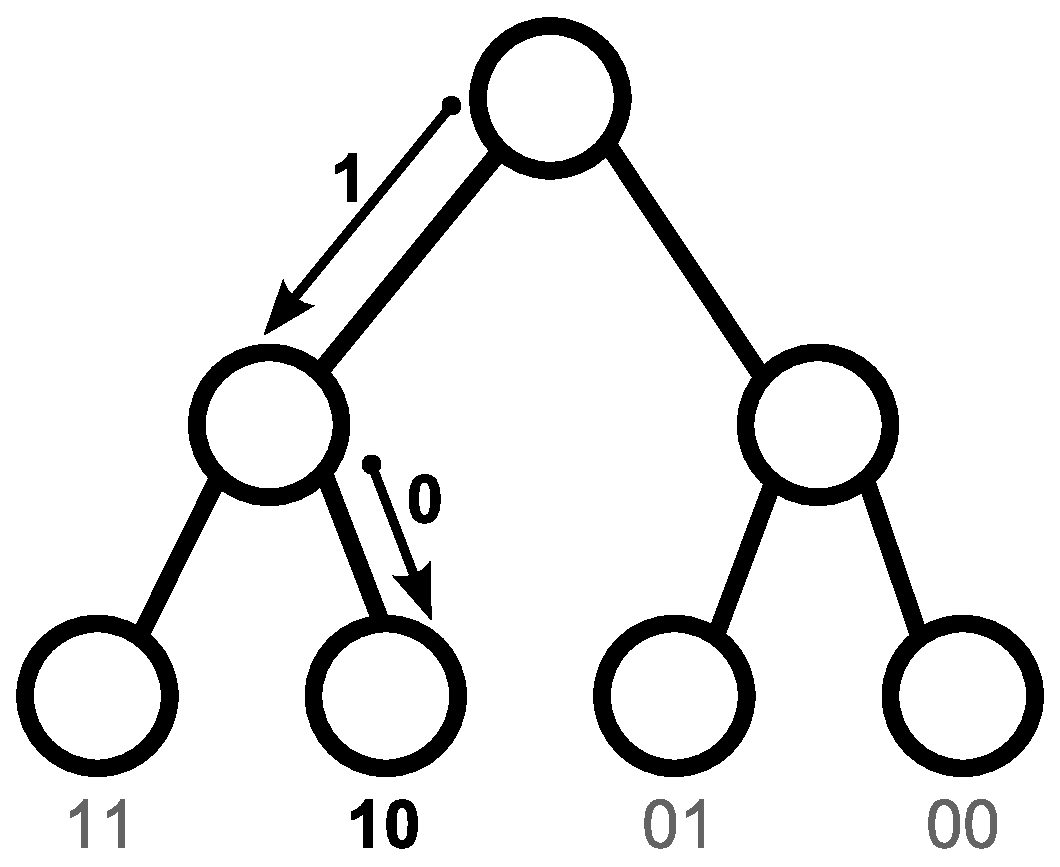
\includegraphics[scale=0.5]{inkscape/tree6.eps}
\caption{Example of a binary tree}
\label{tree6}
\end{figure}
As we cannot uniquely identify $N$ nodes with binary words all of length $< \left\lfloor \log N \right\rfloor$, there is at least one path of length $> \log N$.
\end{proof}

\begin{theorem}
No deterministic sorting algorithm can sort $n$ entries (with just comparisons) in $o(n\log n)$ worst case scenario.
\end{theorem}
\begin{proof}
Build the decision tree (see Figure \ref{tree7}) from the sequence of questions to be asked to the data (the comparisons).
\begin{figure}[htbp]
\centering
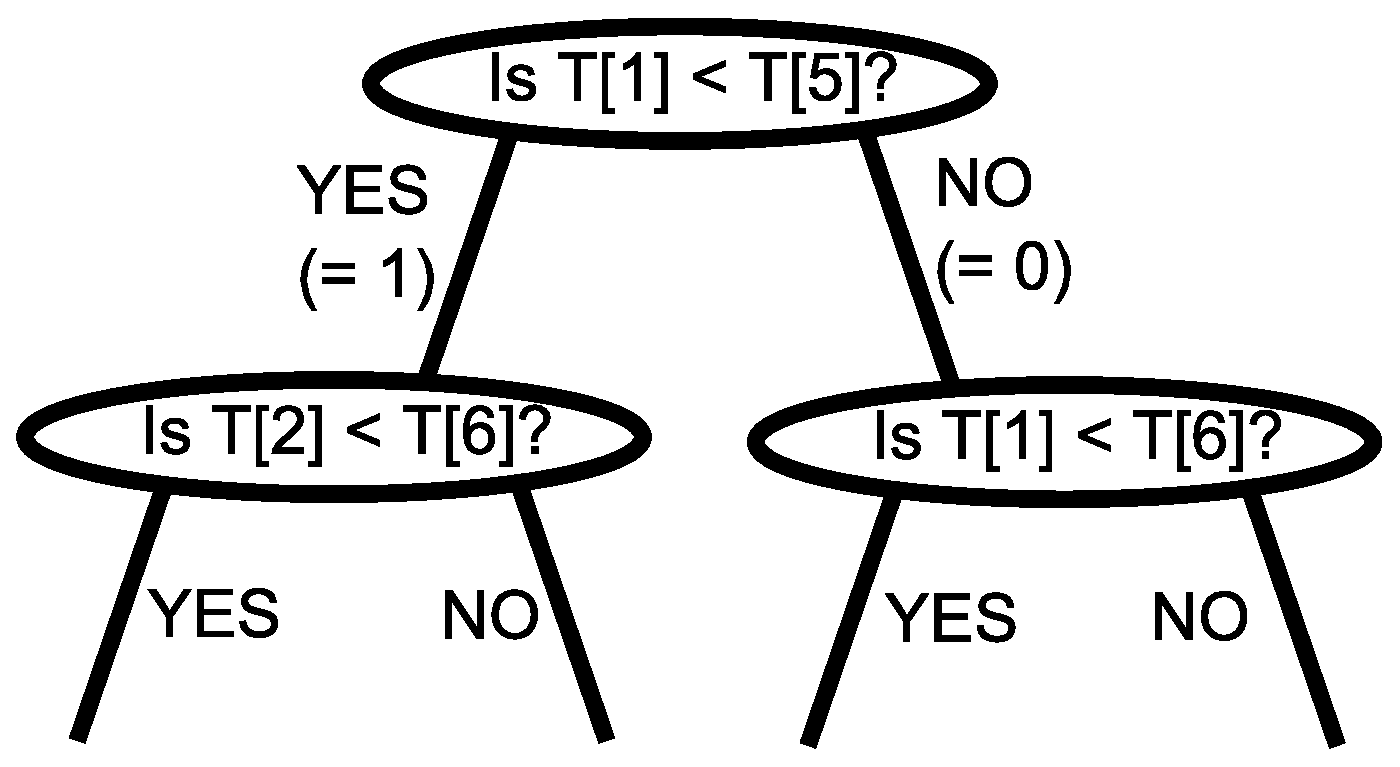
\includegraphics[scale=0.5]{inkscape/tree7.eps}
\caption{Decision tree}
\label{tree7}
\end{figure}
The number of leaves of this tree is $n! = n(n-1)(n-2)...1$. This is the number of possible orders of the input array, each of which will require a different sequence of decisions (leading to different answers to the questions, as the algorithm is deterministic: the same answers leads to the same actions on the data). \\ \\
$\Rightarrow \exists$ one path of length $\log (n!)$ and thus $\log(n!)$ questions. \\ \\
Using the Stirling approximation $n! = \left( \dfrac{n}{e} \right)^n \sqrt{2\pi n}$, we obtain $\log (n!) = n \log n$. We have thus $\Omega (n \log n)$ as worst case complexity.
\end{proof}

This last theorem answers our question for the worst case scenario, but can the average-case complexity be better? The following theorems will answer that question.

\begin{theorem}[Shannon 1948]
Let an $N$-set be endowed with the probabilistic distribution $\rho_1, \rho_2,..., \rho_N$. Label every entry with a binary word (in a prefix way: no word is a prefix to another). Then the expected length (weighted by $(\rho_i)$) is $\geq \sum_{i=1}^{N} -\rho_i \log \rho_i$. 
\end{theorem}
\begin{theorem}
The average length of a path $\text{root} \rightarrow \text{leaf}$ of a $N$-leaf binary tree, with uniform distribution on leaves, is at least $\sum_{i=1}^N -\dfrac{1}{N} \log \dfrac{1}{N} = \log N$.
\end{theorem}
\begin{theorem}
The average-case complexity of \emph{any} deterministic sorting algorithm using comparisons is $\Omega (n\log n)$.
\end{theorem}
\begin{proof}
Apply previous theorems on decision tree.
\end{proof}

\paragraph*{NB:} Randomized algorithms cannot be better either.

As we now know, with our current hypothesis, we cannot do better than $\Omega (n\log n)$. But with supplementary knowledge, we can beat the $\Omega (n\log n)$ bound.
\\ \\
If we know that the entries $\in \left\{ 1,2,...,k \right\}$, we can define the algorithm CountingSort on $\left[ \text{T(1)} \; \text{T(2)} \; \cdots \; \text{T(}n\text{)} \right]$.

\paragraph*{CountingSort}\begin{enumerate}
\item \begin{itemize} 
	\item Count how many entries $=1 \;$:$\; U(1)$
	\item Count how many entries $=2 \;$:$\; U(2)$
	\item $\qquad \qquad \qquad \vdots$
	\item Count how many entries $=k \;$:$\; U(k)$
	\end{itemize}
\item Create $V = \left[ U(1), U(1)+U(2), U(1)+U(2)+U(3), ..., U(1)+U(2)+\cdots+U(k) \right]$.
\item \begin{itemize} 
	\item Copy entries $=1$ to final array $W(1),...,W(U(1))$.
	\item Copy entries $=2$ to final array $W(U(1)+1),...,W(U(1)+U(2))$.
	\item $\qquad \qquad \qquad \vdots$
	\item Copy entries $=k$ to final array $W(U(1)+\cdots+U(k-1)+1),...,W(U(1)+\cdots+U(k))$.
	\end{itemize}
\end{enumerate}
We have thus the following relations (for $i=n,...,1$):
\begin{align*}
W(V(T(i))) & = T(i) \\
V(T(i)) & = V(T(i)) - 1
\end{align*}

\paragraph*{Complexity} The worst case complexity of this algorithm is $\mathcal{O}(k+n)$, computed as follow:
\[ 
\begin{rcases*}
\text{2 passes on T: } \mathcal{O}(n) \\
\text{Creation of U: } \mathcal{O}(k)
\end{rcases*} \mathcal{O}(k+n)
\]
\paragraph*{Remark} Often an entry is just a key to satellite data (a file, a picture, a book, etc.). In those cases, CountingSort is stable: the order of two entries with the same key values is preserved. They are not swaped in the final array W.

\end{document}
